\documentclass[a4paper,12pt]{report}
%\documentclass[aps,twocolumn,secnumarabic,balancelastpage,amsmath,amssymb,nofootinbib,floatfix]{revtex4-1}
\usepackage[utf8]{inputenc}
\usepackage[a4paper, total={6in, 8in}]{geometry}
\usepackage{graphicx}
\usepackage{mathrsfs}
\usepackage{amsmath}
\usepackage{amsfonts}
\usepackage{sidecap}
\usepackage{setspace}

\renewcommand{\thesection}{\arabic{section}}

\begin{document}

\title{Numerically Solving the Poisson Equation}
\author{Noah Green \\ Michigan State University}
%\affiliation{Michigan State University}
\date{ February 12, 2016}
\maketitle
\begin{abstract}
 It is demonstrated here that the Poisson Equation with Dirichlet boundary conditions can be solved with two different numerical techniques: a general LU decomposition (LU) algorithm and a Gaussian elimination (GE) algorithm for tridiagonal matrices. Comparing the algorithms, it is seen that both generate the same relative error when compared to the analytical solution. However, as the number of steps over the function interval is increased, the GE algorithm computation time increases linearly, while the LU algorithm computation time increases cubically. It is also shown that the relative error of these numerical calculations has a lower limit based on the number of bits available to represent numbers on a specific operating system.
\end{abstract}

\doublespacing
\section{Introduction}
The Poisson Equation is an important equation in physics, especially in classical electromagnetism where it can be used to describe the electromagnetic potential due to some charge distribution. In the electromagnetism case, three-dimensional equation is
\begin{equation}
\label{eq:poisson3}
 \nabla^2\Phi = -4\pi\rho(\boldsymbol{r}),
\end{equation}
where $\rho$ is the charge distribution and $\Phi$ is the electromagnetic potential. It is often difficult or impossible to find an exact analytical solution to equation (\ref{eq:poisson3}). This makes it necessary to find efficient numerical techniques as an alternate method to find a solution. 

Since computers function using a binary operating system, numerical calculations are limited to some interval of a countably infinite set. This makes it necessary to ``discretize'' calculations that are normally performed analytically over $\mathbb{R}$ or $\mathbb{C}$. This can be demonstrated using the one-dimensional Poisson equation with Dirichlet boundary conditions:
\begin{equation}
\label{eq:poisson1}
 -\dfrac{d^2u}{dx^2} = f(x), \; x\in(0,1), \; u(0) = u(1) = 0.
\end{equation}
The $u(x)$ function can be made discrete over $n$ subintervals by creating a vector of its values at the boundary of each subinterval ( aka grid points ). Let the length of each subinterval be $h = 1/(n+1)$. Then the $i^{th}$ grid point is $x_i = i*h$. Let $u_i = u(x_i)$, then the discretized vector version of $u(x)$ is
\begin{center}
 $\boldsymbol{u} =
\begin{pmatrix}
  u_1\\
  \vdots\\
  u_{n}
\end{pmatrix}.$
\end{center}
Using the definition of the first and second derivatives, an approximation to the Poisson equation at the $i^th$ grid point can then be defined by
\begin{equation}
\label{eq:poissond}
 -\frac{u_{i+1} + u_{i-1} - 2u_i}{h^2} = f_i,
\end{equation}
where $f_i = f(x_i)$ \cite[ch.~7]{Landau:2008}. This can be rearranged for all $i = 1,...,n$ and expressed by a linear set of equations
\begin{equation}
 \label{eq:laprob}
  \boldsymbol{M}\boldsymbol{u} = \boldsymbol{b},
\end{equation}
where $\boldsymbol{b} = h^2\boldsymbol{f}$ and 
\begin{equation}
\label{eq:tridiag}
\boldsymbol{M}=
 \begin{pmatrix}
    2      & -1 &  0 & \cdots & \cdots  & 0  \\
   -1      &  2 & -1 &   0    & \cdots  & 0  \\	
    0      & -1 &  2 &   -1   & \ddots  & 0  \\
    \vdots &  \ddots &  \ddots &   \ddots   & \ddots  & \vdots  \\
    0      & \cdots &  \cdots &  -1   & 2  & -1 \\
    0      & \cdots &  \cdots &  0   & -1  & 2 
 \end{pmatrix}.
\end{equation}
Hence, solving the Poisson equation numerically amounts to finding an algorithm that will solve equation (\ref{eq:laprob}) for $\boldsymbol{u}$.

\section{Methods for Calculations}
The algorithms used here to calculate the solution of the Poisson equation used a source term $f(x) = 100e^{-10x}$. The analytical solution for the Poisson equation with boundary conditions as in equation (\ref{eq:poisson1}) is given by $u(x) = 1-(1-e^{-10})x-e^{-10x}$.
\subsection{Algorithm: Tridiagonal Gaussian Elimination}
The first algorithm used was a Gaussian elimination (GE) method. When it is reduced to a case-specific algorithm for tridiagonal matrices only, it becomes very efficient, requiring only $O(8n)$ FLOPS. It is achieved by using basic row reduction operations on the matrix in equation (\ref{eq:tridiag}). These operations are:
\begin{enumerate}
 \item Swapping two rows.
 \item Multiplying a row by a nonzero constant.
 \item Adding a multiple of one row to another.
\end{enumerate}

Operation $(1)$ would be used to get a zero value off of the main diagonal. Only operations $(2)$ and $(3)$ are necessary for a well behaved tridiagonal matrix such as equation (\ref{eq:tridiag}). For an $n\times n$ tridiagonal matrix, the following algorithm is used to solve equation (\ref{eq:laprob}).

\singlespacing
\begin{verbatim}
   // ---------start algorithm------------

  // temporary vector for algorithm
  vect<double> vect_temp( _N+1, 0. );

  // forward substitution
  double b_temp = tri_b.get(1);
  _csolution.set( 1, _ctwidd.get(1)/b_temp );
  for( int i = 2; i < _N+1; i++){
    vect_temp.set( i, tri_c.get(i-1)/b_temp );
    b_temp = tri_b.get(i) - tri_a.get(i)*vect_temp.get(i);
    _csolution.set( i, 
		    ( _ctwidd.get(i) - _csolution.get(i-1)*tri_a.get(i) )
		    /b_temp);
  }

  // backwards substitution
  for( int i = _N-1; i >= 1; i-- ){
    _csolution.set( i, _csolution.get(i) 
		    - vect_temp.get(i+1)*_csolution.get(i+1) );
  }

  // Ensure boundary conditions
  _csolution.set(0,0.);
  _csolution.set(_csolution.length()-1,0);

  // -----------end algorithm-------------

\end{verbatim}
\doublespacing

Here, from equation (\ref{eq:laprob}), $tri\_a$, $tri\_b$, and $tri\_c$ are the nonzero diagonals of the matrix $\boldsymbol{M}$, $\_ctwidd$ is $\boldsymbol{b}$, and $\_csolution$ is $\boldsymbol{u}$.

\subsection{Algorithms: LU Decomposition and General Gaussian Elimination}

The general Gaussian elimination algorithm is \textit{much} slower than that for tridiagonal matrices only ($O(8n)$ vs $O(2/3n^3)$. One forward substitution can clear all of the nonzero values below one of the diagonals, so $n$ forward substitutions are required to get an upper triangular matrix. A final backwards substitution can clear all nonzero values above the main diagonal, meaning the calculation time for the algorithm increases as the cube of the dimension of a square matrix. 

It also solves a general system of linear equations at the same number of FLOPS that general LU decomposition takes to get its upper and lower triangular matrix factors: both algorithms take $O(2/3n^3)$ to complete. However, the LU decomposition (LU) algorithm has the advantage of also easily producing the matrix inverse and determinant along with the solution to the linear system with only a $O(n^2)$ backwards substitution. The LU decomposition algorithm was implemented for this project through the library functions provided by reference \cite{Dux:2016}.

\section{Results of Calculations}

\begin{table}[h]
 \centering
\begin{center}
\begin{tabular}{|c|c|c|c|}\hline
\textbf{Algorithm} & \textbf{Grid Points} & \textbf{Time ( s )} & \textbf{Max Error}\\\hline
LU & 10 & $9.0\times 10^{-6}$ & -0.69\\\hline
GE & 10 & $1.0\times 10^{-6}$ & -0.69\\\hline
LU & 100 & $2.2\times 10^{-3}$ & -3.1\\\hline
GE & 100 & $1.0\times 10^{-5}$ & -3.1\\\hline
LU & 1000 & 9.6 & -5.1\\\hline
GE & 1000 & $9.0\times 10^{-5}$ & -5.1\\\hline
LU & 10000 & $3484$ & -7.1 \\\hline
GE & 10000 & $8.9\times 10^{-4}$ & -7.1\\\hline
\end{tabular}
\end{center}
\caption{Table of computation times and $log_{10}$ of maximum relative errors for various numbers of subdivisions for the LU and GE algorithms.\label{tbl:AlgStat}}
\end{table}


These calculations were performed on a 64 bit operating system with 12 gigabytes of RAM and a 2.67 GHz processor. Both the LU and GE algorithms gave decent approximations to the solution of the Poisson equation using only 10 grid points with a maximum relative error of $10^{-.69}\approx20\%$. It can be seen in figure \ref{fig:SCGE10} that this error is likely due to trying to approximate a line with a decent amount of curvature, $u(x) = 1-(1-e^{-10})x-e^{-10x}$, with relatively long straight line segments. 

\begin{SCfigure}
\centering
 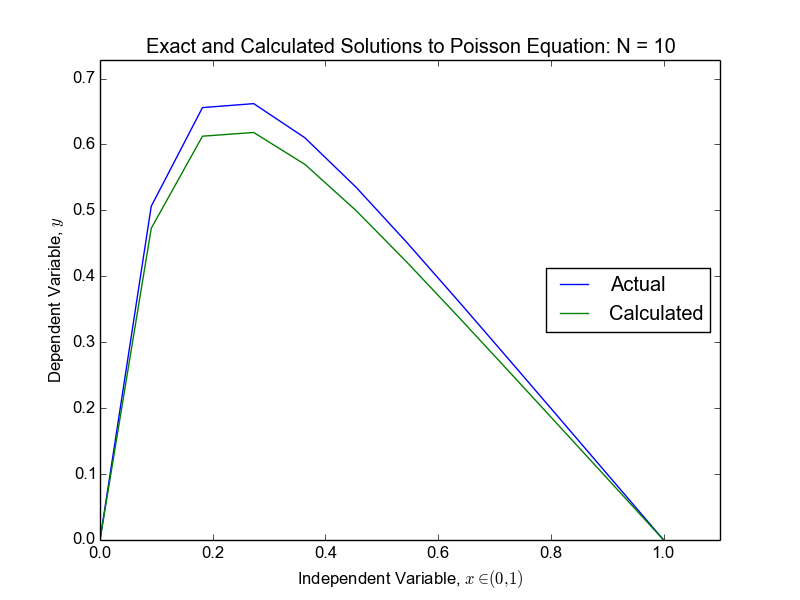
\includegraphics[width=0.5\textwidth]{SolutionCoords_GDG_N10.png}
 \caption{Plot of analytical and calculated solutions for $N=10$.}
 \label{fig:SCGE10}
\end{SCfigure}

This difference becomes indiscernible for larger numbers of grid points, as in figure \ref{fig:SCGE1000} with $N = 1000$.

\begin{SCfigure}
\centering
 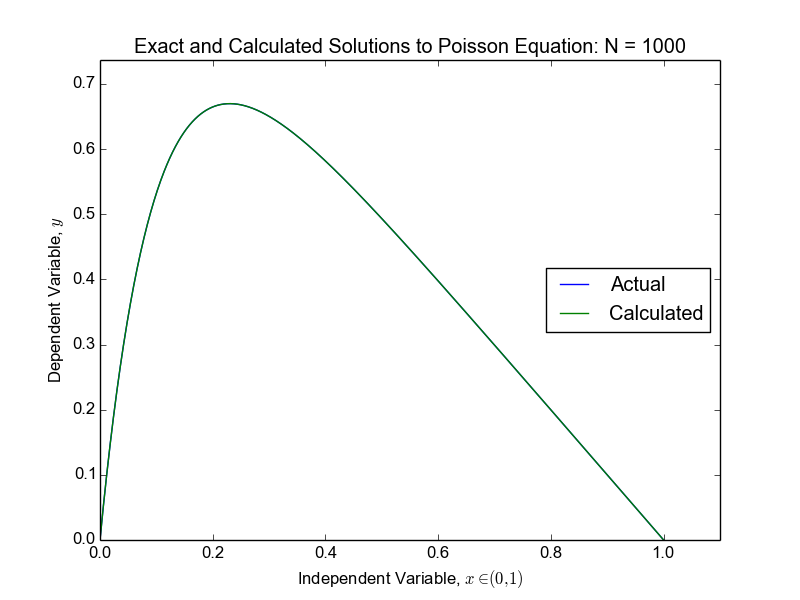
\includegraphics[width=0.5\textwidth]{SolutionCoords_GDG_N1000.png}
 \caption{Plot of analytical and calculated solutions for $N=1000$.}
 \label{fig:SCGE1000}
\end{SCfigure}

Looking at table \ref{tbl:AlgStat}, both algorithms give exactly the same result with the error falling off as approximately $10N^{-2}$. This result can be seen graphically for additional data points in figure \ref{fig:EvNB}. 

However, the FLOPS of each algorithm differentiates them drastically. With 10000 grid points, the specialized GE algorithm still only took about a millisecond to complete, while the general LU algorithm took nearly an hour. This is consistent with the expected increase in computation time. Looking at figure \ref{fig:TvsN}, the GE algorithm increases linearly while the LU algorithm increases cubically, as expected.

\begin{SCfigure}
\centering
 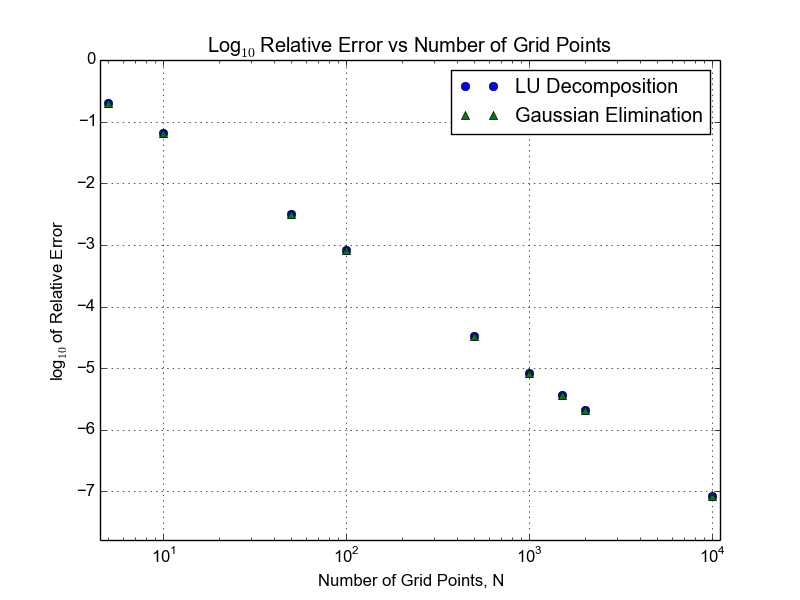
\includegraphics[width=0.5\textwidth]{ErrorVsNPlotBoth.png}
 \caption{Plot of the $log_{10}$ of the relative error vs the number of steps. Note that both algorithms give the same results.}
 \label{fig:EvNB}
\end{SCfigure}

\begin{SCfigure}[][lh]
\centering
 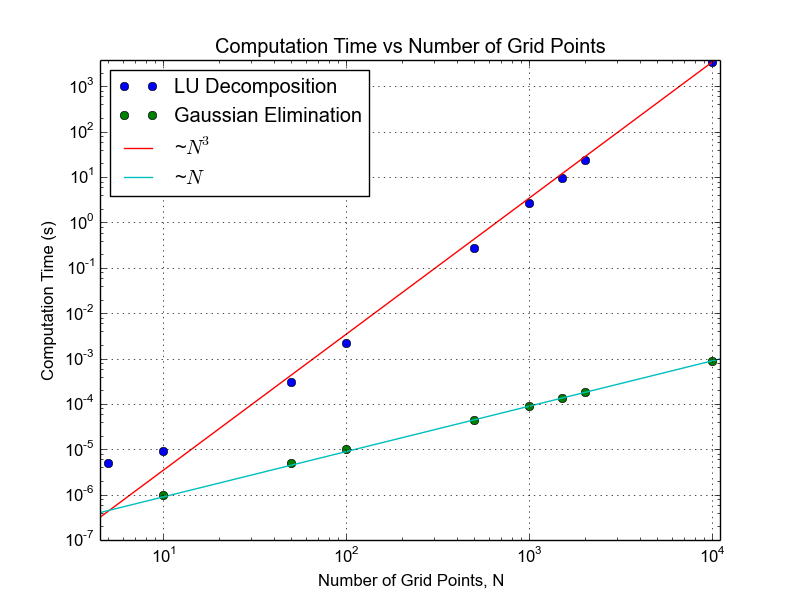
\includegraphics[width=0.5\textwidth]{TimeVsNPlot.png}
 \caption{Plot of time to complete each algorithm vs number of steps.}
 \label{fig:TvsN}
\end{SCfigure}


Lastly, it can be seen in figure \ref{fig:EvNL} that the relative error of the GE algorithm stops decreasing at around 125000 grid points and becomes erratic. Note this was not done for the general LU algorithm due to computation time and memory limitations. This is evidence that the algorithm is encountering numbers where the difference between them is less than the accuracy of a double (~15 digits).

\begin{SCfigure}[][lh]
\centering
 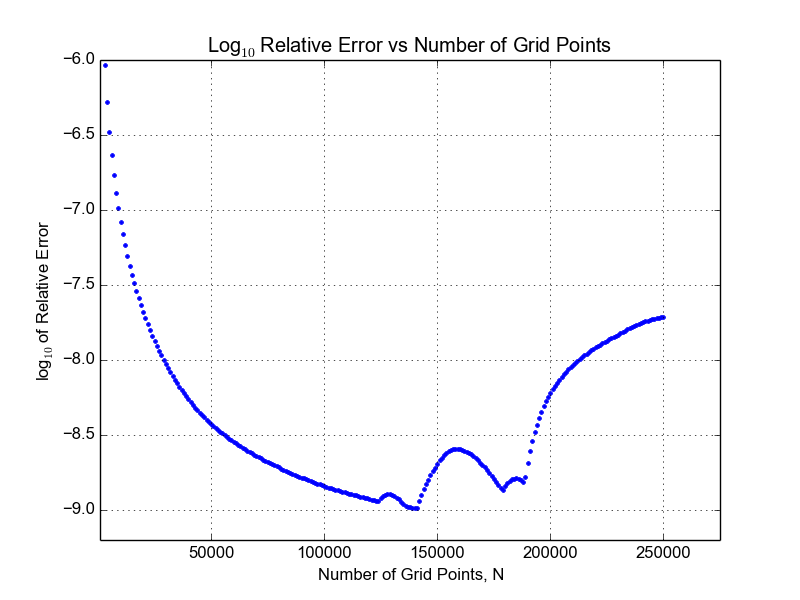
\includegraphics[width=0.5\textwidth]{ErrorVsNPlotLimit.png}
 \caption{Plot of the $log_{10}$ of the relative error vs the number of steps. Note that the relative error stops decreasing once $N\sim10^5$.}
 \label{fig:EvNL}
\end{SCfigure}



\pagebreak[2]
\section{Conclusion}
The tridiagonal GE algorithm is clearly better in terms of speed for calculating the numerical solution to the Poisson equation. By only linearly scaling in computation time with the number of grid points, it was possible to push the approximation to the limit of the computer's accuracy with doubles. However, this algorithm will not work for general matrices. 

The massive gains of the specialized algorithm shows that it is wise to use a general numerical solver only in cases where (1) they can complete the calculation in a reasonable amount of time with adequate precision, or (2) a specialized algorithm is not known to exist for the particular problem. 


\nocite{*}
\bibliographystyle{apalike}
\bibliography{ReportProject1.bib}
\end{document}          
